\documentclass[11pt]{article}

\usepackage{ctex}
\usepackage{bookmark}
\usepackage{listings}
\usepackage{epsfig}
\usepackage{lscape}
\usepackage{multirow}
\usepackage{longtable}
\usepackage{amsmath,amssymb,amsthm}
\usepackage{graphicx}
\usepackage{color}
\usepackage{placeins}
\usepackage{url}
\usepackage{cases}
\usepackage{hyperref}
\usepackage{setspace}
\usepackage{subfigure}
\usepackage{float}
\usepackage{framed}
\usepackage[c2]{optidef}
\usepackage{tikz}
\usepackage{caption}
\usepackage{algorithm}
\usepackage{algpseudocode}
\usepackage{endnotes}
\usepackage{fontspec}


\usepackage{booktabs}

\oddsidemargin 0pt
\evensidemargin 0pt
\marginparwidth 10pt
\marginparsep 10pt
\topmargin -20pt
\textwidth 6.5in
\textheight 8.5in
\parindent = 20pt

\DeclareMathOperator*{\argmin}{argmin}
\DeclareMathOperator*{\minimax}{minimax}

\renewcommand{\algorithmicrequire}{ \textbf{function:}}
\renewcommand{\algorithmicreturn}{ \textbf{end function}}
\newcommand{\blue}[1]{\begin{color}{blue}#1\end{color}}
\newcommand{\magenta}[1]{\begin{color}{magenta}#1\end{color}}
\newcommand{\red}[1]{\begin{color}{red}#1\end{color}}
\newcommand{\green}[1]{\begin{color}{green}#1\end{color}}

\newtheorem{theorem}{Theorem}
\newtheorem{proposition}{Proposition}
\newtheorem{lemma}{Lemma}
\newtheorem{corollary}{Corollary}
\newtheorem{remark}{Remark}
\newtheorem{assumption}{Assumption}
\newtheorem{definition}{Definition}
%\newenvironment{proof}{{\noindent\it Proof}\quad}{\hfill $\square$\par}

%\usepackage{sidecap}


\definecolor{codegreen}{rgb}{0,0.6,0}
\definecolor{codegray}{rgb}{0.5,0.5,0.5}
\definecolor{codemauve}{rgb}{0.58,0,0.82}

\lstset{ %
	language=python,                % choose the language of the code
	basicstyle=\footnotesize\ttfamily,       % the size of the fonts that are used for the code
	numbers=left,                   % where to put the line-numbers
	numberstyle=\tiny\color{codegray},      % the size of the fonts that are used for the line-numbers
	stepnumber=1,                   % the step between two line-numbers. If it is 1 each line will be numbered
	numbersep=5pt,                  % how far the line-numbers are from the code
	backgroundcolor=\color{white},  % choose the background color. You must add \usepackage{color}
	showspaces=false,               % show spaces adding particular underscores
	showstringspaces=false,         % underline spaces within strings
	showtabs=false,                 % show tabs within strings adding particular underscores
	frame=single,                   % adds a frame around the code
	tabsize=4,                      % sets default tabsize to 4 spaces  
	captionpos=b,                   % sets the caption-position to bottom
	breaklines=true,                % sets automatic line breaking
	breakatwhitespace=false,        % sets if automatic breaks should only happen at whitespace
	escapeinside={\%*}{*)},
	commentstyle=\color{codegreen},
	keywordstyle=\bfseries\color{magenta},
	stringstyle=\color{red},
	identifierstyle=\color{codemauve},
	keepspaces=true
}


\begin{document}

\title{\bf Lab 2 实验报告}

\author{}
\date{\today}
\maketitle


\section{问题描述}

在 Lab 0 中,我们利用递归方式回溯 LCS 所有结果的输出,但输出过程中存在重复,为了去重我们采用了 set 数据结构,
这是一种计算开销很大的算法。例如如下情况,A = X1234567890 和 B = Xabcdef 只有一个 LCS ,但是按照朴素算法
我们将在每一个节点都进行分岔搜索。面对比较坏的情况,我们将无端多出指数级的开销。

\begin{figure}[H]
	\centering
	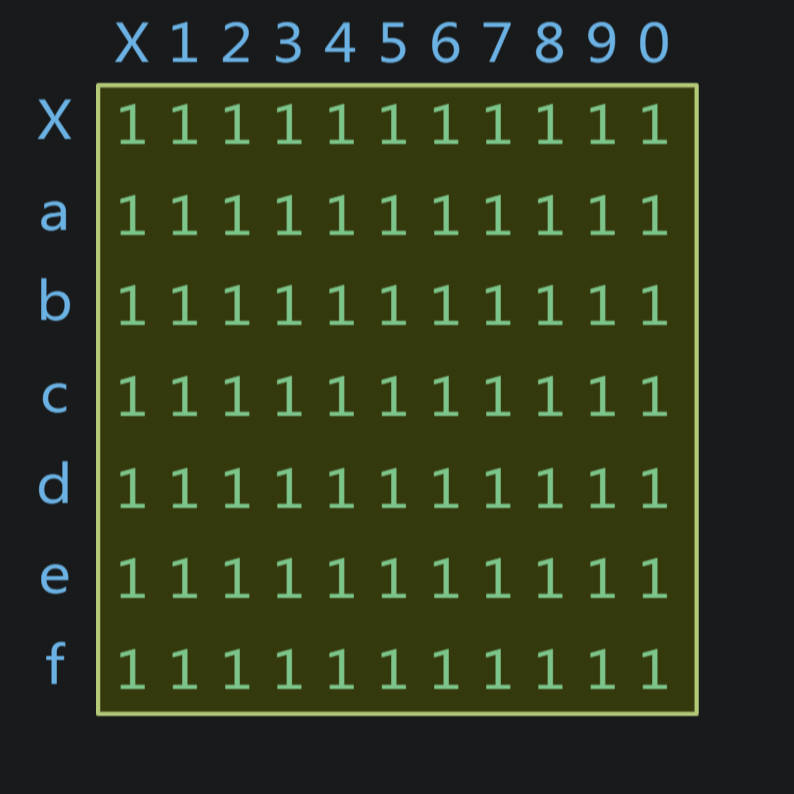
\includegraphics[width=0.5\textwidth]{./img/example.jpg}
	\caption{特殊情况}
\end{figure}

为了解决冗余输出,一种思路是将 LCS 输出的树结构转化为图结构,将相同节点合并。幸运的是,Ronald I. Greenberg
发明了一种能在 $ O(mn) $ 时间开销内将 LCS 二维表压缩为 LCS 图(一种可以表示所有互不相同的 LCS 的图)的算法,
本次实验将基于此算法在图结构上遍历打印所有 LCS 输出。


\section{算法设计}

对任务一,串行打印 LCS Graph 节点,只需唯一且完备遍历所有节点,每次访问时输出即可。常见的解法有 BFS 和 DFS ,
以 BFS 算法为例,关于 lcsNode 的定义以及 Queue 相关算法的具体实现详见 utils ,以下仅展示核心思路。

\begin{algorithm}[H]
	\caption{BFS}
	\begin{algorithmic}
		\State $\textbf{Input}$ graph $G$, source node $s$
		\State $\textbf{Let}$ $Q$ be queue
		\State $Q$.enqueue( $s$ )
		\State mark $s$ as visited
		\While{$Q$ is not empty}
		\State $v$  =  $Q$.dequeue( )
		\For{each neighbour $w$ of $v$ in graph $G$}
		\If{$w$ is not visited}
		\State $Q$.enqueue( $w$ )
		\State mark $w$ as visited
		\EndIf
		\EndFor
		\EndWhile
	\end{algorithmic}
\end{algorithm}

对任务二,串行输出所有 LCS 结果,只需按 DFS 顺序递归调用输出,核心思路如下。

\begin{algorithm}[H]
	\caption{DFS by recursion}
	\begin{algorithmic}
		\State $\textbf{Input}$ file pointer $fp$, LCS output $lcs$, current cell $cell$
		\If{$cell\rightarrow successors$ is not NULL}
		\If{$cell\rightarrow match$ is not NULL}
		\State $lcs$[$cell\rightarrow rank$ - 1] = $cell\rightarrow match$
		\EndIf
		\For{each successor $w$ of $cell$}
		\State DFS( $fp$, $lcs$, $w$ )
		\EndFor
		\Else
		\State print $lcs$ to $fp$
		\EndIf
	\end{algorithmic}
\end{algorithm}

对任务三,要求并行输出所有 LCS 结果。受到 TLS 启示,每个线程使用各自独占的缓存并输出到各自对应的文件,算法设计如下。
假设有 P 个线程,先用如任务一中的 BFS 串行找到至少 P 个分岔,然后将每一个分岔分给线程并且并行执行 (线程执行任务是串
行执行) ,如果还有剩余的分岔则再继续展开,重复上面的过程,直至队列清空或者所有分岔被分完。而当线程切换到新任务时,可
利用双向链表回溯该节点的父节点,以得到此前串行走过的 LCS 路径。


\section{实验结果}

测试输出如下,正常情况下并行输出速度可以达到串行 10 倍左右;而病态例子 (存在大量分岔) 下会出现并行速度慢于串行的情况,
可能原因是例子阶数不够大,导致并行文件读写带来的开销大于并行加速的增益。

\begin{figure}[H]
	\centering
	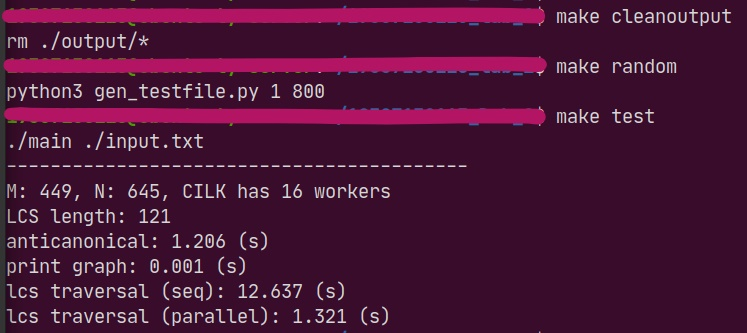
\includegraphics[width=0.5\textwidth]{./img/output-1.jpg}
	\caption{实验结果-正常}
\end{figure}

\begin{figure}[H]
	\centering
	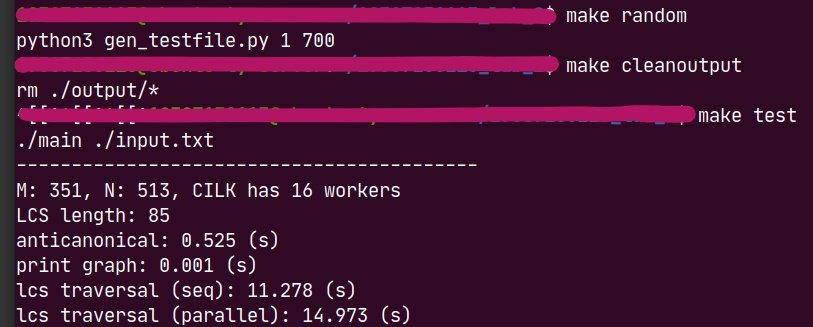
\includegraphics[width=0.5\textwidth]{./img/output-2.jpg}
	\caption{实验结果-反常}
\end{figure}


\end{document}


